In order to test the hypothesis, we first derive a number of questions from the hypothesis.

\begin{itemize}
\item{Improvement in performance can only come from extraction of relations between concepts, since all words are also contained in the plain text underlying the graph.}
\item{Structure of concept maps must bear more information than simple bi- or tri-grams.}
\item{Kernels that only take the labels into account, should perform worse.}
\end{itemize}

\paragraph{Question: ``How similar/diverse are the graphs structurally?"}
If the structure of the graphs is too similar and the structural differences are not distinct between the classes, they most likely will not be that useful for classification.
When comparing the graph similarity with respect to some graph kernel, the graphs in some class should be distinguishable from the graphs in another class.

To explore the differences, we look at three questions in particular:
``How similar are the graphs... $a)$ in the same class, $b)$ between (pairs of) classes and $c)$ in the complete dataset?"

\paragraph{Question: ``How important (relatively) are the labels/structure?"}

\paragraph{Question: ``How does the classification performance compare to classical, non-structural approaches (text based, tfidf?)"}

\paragraph{Question: ``What are possible roadblocks for text classification by using graph classification?}

\paragraph{Question: ``How do the graph kernel parameters, for example the depth of the sub-structures that are considered, affect the classification score?}

\todo{Since we are especially interested in answering structure-related questions about the graphs, we first have to distinguish structural from non-structural data.}
\todo{Explain the used metrics and how they relate to hypothesis}
\todo{Explain the datasets and how they differ, why they are important?}
\todo{Introduce the baselines, explain how they relate to the hypothesis, why they - are chosen, how they differ}
\todo{Explain methodology, why the chosen metric really captures the problem at - hand}
\todo{Work out differences of graph types, find similarities across datasets}
\todo{Provide the questions that are relevant for the hypothesis}
\todo{Answer these questions through metrics/results}

\labelsubsection{Experiments}{subsec:experiments}
\todo{Test the hypothesis}
\todo{Tables with results}
\todo{Mention difficulties and possible solutions}
\todo{Add runtime analysis}

\subsubsection{Baselines}
\paragraph{Preprocessing}
Before creating the vector representations of the text documents or the creation of the co-occurrence graphs and concept maps, we first pre-processed the plain text by

\begin{itemize}
\item{lowercasing the text,}
\item{removing non-printable characters,}
\item{replacing numbers with a \textit{NUMBER} placeholder,}
\item{replacing tabs and newlines with a space,}
\item{and normalizing the whitespace (eg. replacing multiple spaces with a single space)}
\end{itemize}
These pre-processing steps are similar to the pre-processing done in \cite{Cachopo2007}.

\todo{Filtered out only nouns?}

\paragraph{Text-based representations}
For the text classification pipeline, we then used two different vectorization algorithms, namely
\begin{itemize}
\item{Bag Of Words (BoW): this vectorizer simply gathers all words in the corpus and creates a mapping between words and indices (ids). Then it creates a vector representation for each text so that the i-th vector component  is the count of the corresponding word in the text. Ie. $i$ is the index of the word in the mapping.}
\item{Term-Frequency-Inverse-Document-Frequency (TfIdf): this approach is similar to BoW. Instead of using only the counts of a word in the text, this approach also incorporates the term frequency and the inverse document frequency of the words to the vector representation (see below).}
\end{itemize}
Both approaches can also be extended by not only utilizing single words (unigrams) but n-grams, too. N-grams consist of $n$ consecutive words in the text.
For example, the sentence ``This is a sentence." has the following 2-grams, or bigrams: $\{ (This, is), (is, a), (a, sentence) \}$.
For our purposes, we looked at n-grams of lengths (1, 1), (1, 2) and (2, 2).

\todo{Explain ranges of n-grams}
\todo{Explain tfidf}

\paragraph{Graph-based representations}

\todo{Co-occurrence and concept maps}
\todo{Mention filtering by nouns}
\todo{Window sizes}

\subsubsection{Approach}
\todo{Combined}
\todo{Code by Tobias, explain steps}

\begin{figure}[ht]
\centering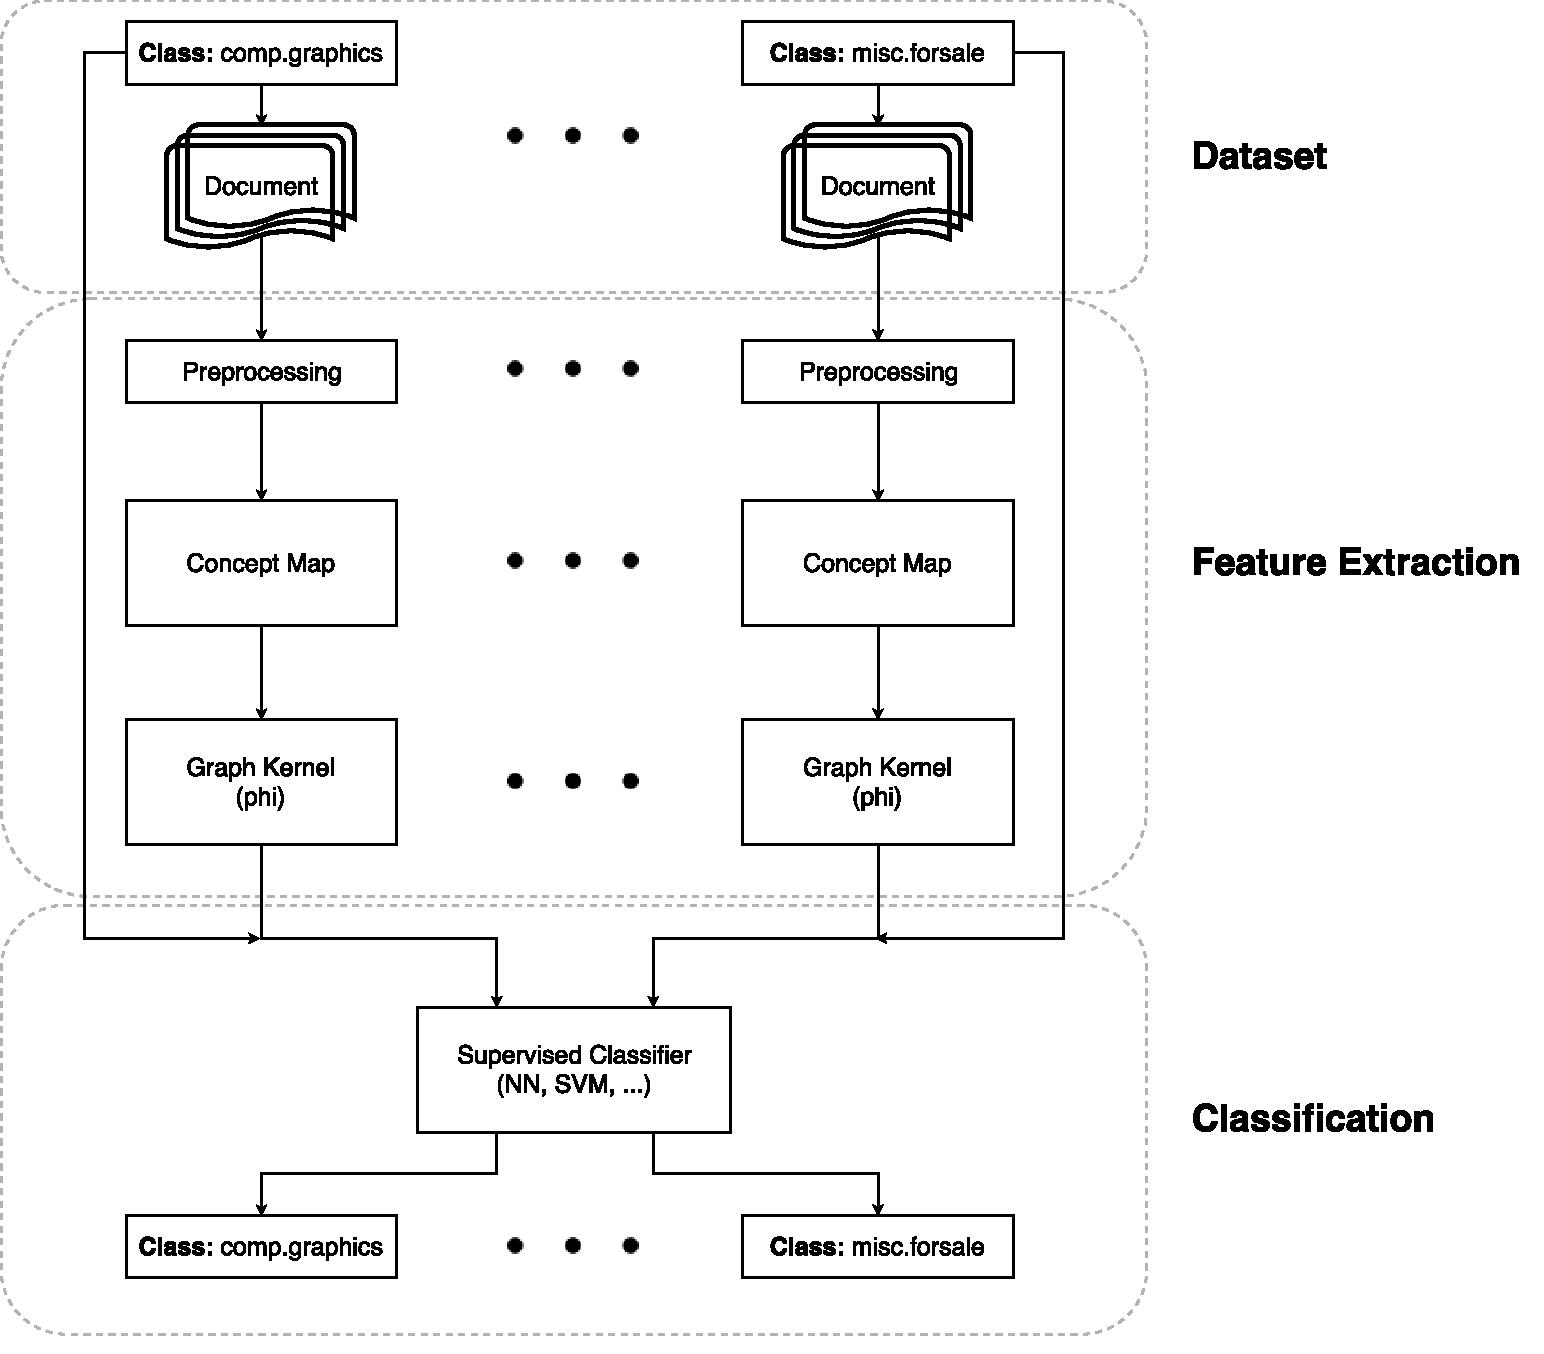
\includegraphics[width=0.6\linewidth]{assets/figures/approach.pdf}
\caption{\todo{Caption}}
\end{figure}
\todo{Add diagram for gram-matrix based classification.}

\labelsubsection{Datasets}{subsec:datasets}
\todo{Statistics about datasets and derived graphs}
\todo{Skewed classes}
\todo{Graph statistics}
\todo{Give hints where to download the datasets from}
\todo{A script to download all datasets is also provided alongside the other code}

\paragraph{ling-spam}
The Ling-Spam dataset was created by Ion Androutsopoulos et al. \cite{Androutsopoulos2000}.
The corpus contains the texts, which are categorized as ``spam" and ``no spam". For this work, we used the version which can be downloaded from here\footnote{\url{http://csmining.org/index.php/ling-spam-datasets.html}}.

\paragraph{ng20}
The 20 Newsgroup corpus consists of newsgroup documents. They are labeled with 20 different classes, corresponding to the newsgroup boards they have been posted on. The texts are mostly informal and consist of discussions between members of a newsgroup.

\todo{Removed headers and footers}
\todo{It has to be noted that some classes are highly correlated}

\paragraph{reuters-21578}
\footnote{\url{http://www.nltk.org/book/ch02.html#reuters-corpus}}
\todo{Documents came from Reuters newswire in 1987.}

\paragraph{r8}
This dataset is a subset of the \textit{reuters-21578} dataset. The 8 most frequent classes, ie. the classes with the most instances, have been filtered out of the \textit{reuters-21578} dataset.

\paragraph{review\_polarity}
\cite{Pang2004}.
\url{http://www.cs.cornell.edu/people/pabo/movie-review-data/review_polarity.tar.gz}

\paragraph{rotten\_imdb}
\cite{Pang2004}.
\url{http://www.cs.cornell.edu/people/pabo/movie-review-data/rotten_imdb.tar.gz}

\paragraph{tagmynews}
\url{http://acube.di.unipi.it/repo/news.gz}

\paragraph{webkb}
\url{http://www.cs.cmu.edu/afs/cs/project/theo-20/www/data/}

\begin{figure}[ht]
\centering
\begin{tabular}{lrr}
dataset &  \# classes &  \# documents \\
\midrule
ling-spam       &  2 &  2893 \\
ng20            &  20 &  18846 \\
r8              &  8 &  9459 \\
reuters-21578   &  90 &  13328 \\
review\_polarity &  2 &  2000 \\
rotten\_imdb     &  2 &  10000 \\
tagmynews       &  7 &  32600 \\
webkb           &  7 &  8274 \\

\end{tabular}

\caption{Dataset statistics}
\end{figure}

\todo{Add statistics about concept maps/co-occurrence graphs (like avg. nodes, avg. edges)}

\labelsubsection{Methods}{subsec:methods}
\todo{Combined}
\todo{Scaler}
\todo{Merging nodes?}

\subsubsection{Cross-Validation}
\subsubsection{Metrics}
\subsubsection{Significance tests}

\labelsubsection{Implementation}{sec:implementation}
\todo{Scikit-learn, networkx, \dots}
\todo{Code by Tobias to extract concept maps}
